% !TEX program = xelatex

\documentclass[8pt,aspectratio=169,mathserif,UTF8]{beamer}		
\usepackage{cqubeamer}  % cqu beamer template

\usepackage{fontspec} % 设置英文字体
\setmainfont{Palatino Linotype} % fontspec宏包下设置全局默认英文字体
%\newcommand{\Centaur}{\fontspec{Centaur}} %单独设置某一字体

\usepackage{xeCJK} %设置中文字体
\setCJKmainfont{STKaiti} %xeCJK宏包下设置全局默认中文字体,默认为楷体STKaiti

\usepackage{amsmath,amsfonts,amssymb,bm}   % 数学公式字体宏包
\usepackage{mathpazo}

\usepackage{xcolor}			               % 颜色宏包
\definecolor{cqu_blue}{RGB}{36,72,164}     % 自定义颜色
\usepackage{adjustbox}

\usepackage{listings}                      % 列表环境
\usepackage{verbatim}



\usepackage[listings]{tcolorbox}
\newtcbox{\mybox}{colback=red!5!white,colframe=green}
\tcbuselibrary{breakable}                  % tcolorbox 跨页显示
\usepackage{graphicx,url}

\usepackage{fontawesome}                   % 矢量图标库宏包
\usepackage{multicol}                      % 多栏显示宏包

\graphicspath{{figure/}} % 定义所有的图片文件在 figure目录下


\begin{document}
\pdfbookmark[1]{CQU Beamer Template}{title} % "1" = section level,书签标题
\beamertemplatenavigationsymbolsempty
 
\title{ CQU Beamer Template}	     %若需要调整背景框长度,请修改cqu.sty中第154行即可
%\subtitle{}
\author[万震(重庆大学)]{
万\ 震\\
\vskip5pt
{\color{blue}\faEnvelopeO}\hspace{0.1cm}{\it{wanzhen@cqu.edu.cn}}\\
{\color{blue}\faGithub}\hspace{0.1cm} {\href{https://github.com/Godblesswz}{Godblesswz}}
\vskip5pt
重庆大学\\
  \begin{center}
  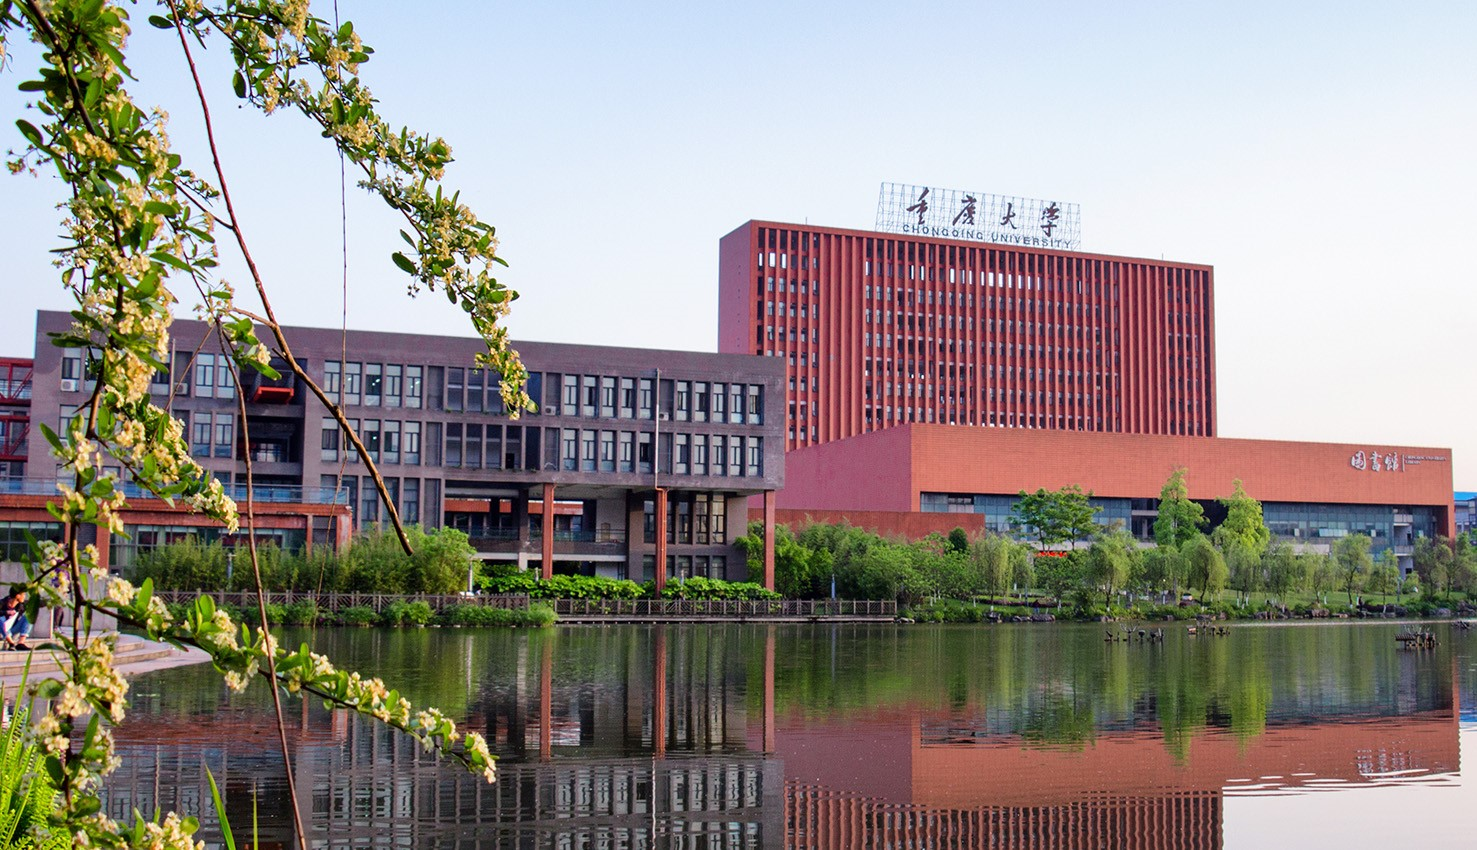
\includegraphics[width=0.4\textwidth]{CQU_Campus_D.jpg}%  
  \end{center}
  \vskip-35pt
}

\date[2018年5月]{2018年5月\quad 重大}
 
% 标题页
\begin{frame}[plain]
  \vskip25pt
  \titlepage
\end{frame}
\setcounter{framenumber}{0}				

% 目录页
\section*{}   
\begin{frame}{目录}
  \begin{multicols}{2}
    \tableofcontents[subsubsectionstyle=hide]  
  \end{multicols}
\end{frame}			

% 正文
\section{CQUBeamer的使用说明}
\subsection{LaTeX 的安装}
\begin{frame}
  \frametitle{LaTeX 的安装}
     \begin{itemize}
      \item MacTeX (Mac OSX), TeXLive (Unix,Linux,Windows), MiKTeX(Windows)
      \item 下载 MacTeX 或 TeXLive 并安装:
         \begin{itemize}
          \item 清华大学 TUNA 协会:\href{https://mirrors.tuna.tsinghua.edu.cn/}{https://mirrors.tuna.tsinghua.edu.cn/}
           \item CTAN: \href{http://www.ctan.org}{http://www.ctan.org}
          \item  CTeX: \href{http://www.ctex.org}{http://www.ctex.org}
         \end{itemize}
      \end{itemize}
\end{frame}

\subsection{CQUBeamer的结构}
\begin{frame}
  \frametitle{CQUBeamer的结构}
  \begin{columns}
   \begin{column}{.35\textwidth}
     \begin{itemize}
      \item 全局基本结构 \verbatiminput{demo_code/demo_layout.tex}
      \item 标题、作者、日期 \verbatiminput{demo_code/demo_titlepage.tex}
      \end{itemize}
   \end{column}

	\begin{column}{.65\textwidth}
     \begin{itemize}
      \item 文档格式 \verbatiminput{demo_code/demo_format.tex}
      \item 文章内容结构\\
      \begin{tabular}{lll}
      结构指令 & 层级 & 备注\\
      $\backslash$part & -1 & 不存在 letters 格式中\\
	   $\backslash$chapter & 0 & 在 books 或 reports 格式中才有\\
	   $\backslash$section & 1 & 不存在 letters 格式中\\
	   $\backslash$subsection & 2 & 不存在 letters 格式中\\
	   $\backslash$subsubsection & 3 & 不存在 letters 格式中\\
	   $\backslash$paragraph & 4 & 不存在 letters 格式中\\
	     & &\\
	   $\backslash$section*  & NULL & 不计数⼊结构层数中
      \end{tabular}
      
      \item 每一帧幻灯片 (可以包括多页)\\
      $\backslash$begin\{frame\}\\
      ......\\
      $\backslash$end\{frame\}
      
      \end{itemize}
	\end{column}
	\end{columns}
\end{frame}

\subsection{CQUBeamer的编译}
\begin{frame}
  \frametitle{CQUBeamer的编译}
     \begin{itemize}
      \item 编译方式: XeLaTeX,可直接用电脑里字体,UTF8 编码。
      \item 中英文字体设置:\verbatiminput{demo_code/demo_fontsetting.tex}
      \end{itemize}
\end{frame}


\section{总结}
\begin{frame}
\frametitle{总结}
\begin{itemize}
  \item 简短地介绍了CQUBeamer的基本结构及其编译方式。
  \item 如果有进一步问题,欢迎与我讨论交流。
  \item 作为热爱\LaTeX 的重大人,在前人的基础上开发了此``CQU Style''的Beamer,希望对有志于采用\LaTeX Beamer 做学术报告的重大人或多或少有些帮助。
  \item 祝所有重大人,在生活和学术之路上,带着自信,大步前行,顺顺利利。
\end{itemize}

\begin{figure}[!htbp]
\begin{center}
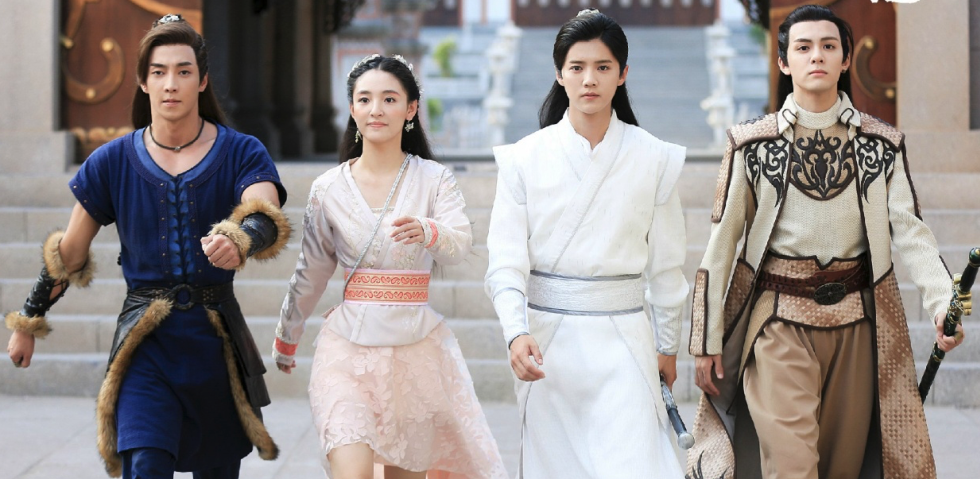
\includegraphics[width=0.5\textwidth]{go.png}
\end{center}
\end{figure}
    
\end{frame}




\section{致谢}

\begin{frame}
\frametitle{致谢}

本CQUBeamer在\href{https://github.com/YLiu1231}{YLiu1231}的\href{https://github.com/YLiu1231/njumath_beamer}{njumath\_beamer}的基础上进行二次开发而成,CQU Log采用\href{https://github.com/CQUtug}{重庆大学TeX用户组}制作的\href{https://github.com/CQUtug/CQULogo}{重庆大学视觉标识素材包},在此向其个人、开发组以及文档中引用了但未明确致谢的版权所属方表示衷心感谢!\vspace{0.5cm}

赠人玫瑰,手留余香!

\end{frame}



\appendix
%\backupbegin
\section*{backup}

\begin{frame}{Back up}
\vskip20pt
\begin{center}
\Huge{谢谢!\\ 欢迎指正和交流分享!}
\end{center}
\vskip20pt
\begin{table}
\begin{tabular}{l}
Zhen Wan (万震) \\
{\color{blue}\faMapMarker}\hspace{0.1cm} School of Civil Engineering, Chongqing University\\
\hspace{0.28cm} No.83 Shabei Street, Shapingba District \\
\hspace{0.28cm} Chongqing, 400045, P. R. China \\
{\color{blue}\faEnvelopeO}\hspace{0.1cm} {\href{mailto:wanzhen@cqu.edu.cn}{wanzhen@cqu.edu.cn}}\\
{\color{blue}\faGithub}\hspace{0.1cm} {\href{https://github.com/Godblesswz}{Godblesswz}}\\
\end{tabular}
\end{table}%
\begin{picture}(0,0)
        \put(30,8){
\includegraphics[width=0.16\textwidth]{Wechat.png}}%
\end{picture}
\end{frame}

%\backupend



\end{document}
